\documentclass[11pt,letterpaper]{article}

\input{../../../../.config/latex/preamble_v1.tex}
\lightmode

\title{\textbf{Math 55b Problem Set 1}}

\begin{document}
\maketitle

\begin{center}
    \textit{I collaborated with AJ LaMotta on this problem set, and it took me about 15 hours.}
\end{center}

% Problem 1
\begin{problem}\noindent
    \begin{enumerate}[(a)]
        \item Use the triangle inequality to show that a sequence $p_1, p_2, p_3, \ldots$ of points in a metric space $X$ can have at most one limit.
        \item Show that any sequence with a limit is Cauchy.
        \item Show by example that the converse isn't true; a Cauchy sequence in a metric space need not have a limit.
        \item We say that a metric space is {\em complete} if every Cauchy sequence has a limit. Find an example of a complete metric space.
    \end{enumerate}
\end{problem}

\begin{changemargin}{1em}{1em}
    \textbf{(a)} Let $(X, d)$ be a metric space and $p_1,p_2,p_3,\ldots$ be a sequence. Suppose for the sake of contradiction that $L_1$ and $L_2$ are two distinct limits of this sequence. Since $L_1\neq L_2$, the distance between them must be positive, say $d(L_1, L_2)=\delta$. Now let $\epsilon>0$ be arbitrary. By the definition of convergence, there must be $n,m\in \N$ such that for every $N \geq n$ and $M\geq m$, $d(p_N, L_1) < \epsilon$ and $d(p_M, L_2) < \epsilon$. Let $i \geq \max(n,m)$ so that $d(p_i, L_1)<\epsilon$ and $d(p_i, L_2)<\epsilon$. Thus by the triangle inequality, we have
     \[
        \delta = d(L_1, L_2) \leq d(p_i, L_1) + d(p_i, L_2) \leq 2\epsilon
    .\] 
    So $\delta\leq 2\epsilon$ for arbitrary $\epsilon$. This is impossible, since $\lambda$ would have to be zero. So $L_1=L_2$.

    \textbf{(b)} Let $p_1,p_2,p_3,\ldots$ be a sequence converging to $L$. To prove that this sequence is Cauchy, let $\epsilon > 0$ be arbitrary. By definition of convergence, there exists  $n\in \N$ such that for all  $N\geq n$,  $d(p_N, L) < \epsilon$. For any other  $M\geq n$,  $d(p_M, L) < \epsilon$, so by the triangle inequality, we have
    \[
        d(p_N, p_M) \leq d(p_N, L) + d(p_M, L) \leq 2\epsilon
    .\] 
    Since $\epsilon$ was chosen arbitrarily, we can scale so that $d(p_N, p_M)\leq \epsilon$, and this will hold true for all  $N, M\geq n$. Thus  $p$ is a Cauchy sequence.

    \textbf{(c)} Consider $\Q$ as a metric space with the standard Euclidean metric. Pick any irrational number $\alpha\in \R$ and let $\alpha_i\in \Q$ be the rational truncation of the decimal expansion of $\alpha$ to $i$ digits after the decimal point. 
    It is clear that $\{\alpha_i\}_i$ is a Cauchy sequence in $\Q$, indeed for any $\epsilon > 0$, let $k\in N$ be such that $\frac{1}{10^k}\leq \epsilon$. 
    Then for every $N,M \geq k+1$, $d(\alpha_N, \alpha_M) < \frac{1}{10^k} \leq \epsilon$. So it is a Cauchy sequence. 
    To see that it does not converge to any limit in $\Q$, note that if $L\in \Q$ was some limit of $\{\alpha_i\}_i$, then $L$ would also be a limit when $\{\alpha_i\}_i$ is considered in the metric space  $\R$. 
    However, as (a) established, limits in metric spaces are unique, so $L$ clearly must be  $\alpha$. However  $\alpha$ is by definition not in $\Q$, so the sequence has no limit in  $\Q$.

    \textbf{(d)} The trivial metric space containing a single point is clearly complete. Unfortunately, this isn't a very interesting space. A more interesting complete space is the real numbers, although this is trickier to prove.
\end{changemargin}

% Problem 2
\begin{problem}\noindent
    \begin{enumerate}[(a)]
        \item Use the triangle inequality to show that open ball is indeed open.
        \item Show that a finite intersection of open subsets in a metric space is open; and that an arbitrary union of open subsets is open.
        \item Deduce from part (b) that an arbitrary intersection of closed subsets in a metric space is closed, and a finite union of closed subsets is closed.
        \item Show by example that an arbitrary intersection of open subsets need not be open.
    \end{enumerate}
\end{problem}
\begin{changemargin}{1em}{1em}
    \textbf{(a)} Let $x\in X$, and $\epsilon > 0$ so that $B_\epsilon(x)$ is an open ball, defined
    \[
        B_\epsilon(x) = \{b\in X \mid d(b,x) < \epsilon\}
    .\] 
    To prove that this ball is indeed an open set, suppose $b\in B_\epsilon(x)$ is some arbitrary point. Let $\delta = \frac{\epsilon - d(b,x)}{2}$. We claim that $B_\delta(b)\subset B_\epsilon(x)$.
    Let $b'\in B_\delta(b)$. Then  $d(b', b)< \delta$ and  $d(b, x) < \epsilon$, so
     \[
        d(b', x)\leq d(b', b) + d(b, x) < \delta + d(b,x) = \frac{\epsilon - d(b,x)}{2} + d(b,x) = \frac{\epsilon + d(b,x)}{2} < \epsilon
    .\] 
    Hence, $b'\in B_\epsilon(x)$, and so  $B_{\delta}(b)\subset B_\epsilon(x)$.

    \textbf{(b)} To prove that finite intersections of open sets are open, it suffices to show that the intersection of two open subsets is open, and the rest would proceed by induction on the number of sets. 
    Suppose $U_1, U_2$ are open sets. Let $b\in U_1\cap U_2$, and by (a), there must exist $\epsilon_1, \epsilon_2 > 0$ such that $B_{\epsilon_1}(b)\subset U_1$ and $B_{\epsilon_2}(b)\subset U_2$. 
    Let  $\epsilon = \min(\epsilon_1, \epsilon_2)$. 
    Then clearly $B_\epsilon(b)\subset U_1\cap U_2$ since  $B_\epsilon(b)\subset B_{\epsilon_1}(b)\subset U_1$ and  $B_\epsilon(b)\subset B_{\epsilon_2}(b)\subset U_2$. 
    So the intersection of two, and hence finitely many open sets is again open.

    Now let $\{U_\alpha\}_\alpha$ be an arbitrary collection of open subsets of $X$. 
    For any $x\in \bigcup_{\alpha}U_\alpha$, say  $x\in U_\alpha$ for some $\alpha$, the open ball $B_\epsilon(x)$ is contained inside  $U_\alpha$, and hence is contained in the union. So the union is open.

    \textbf{(c)} As in (b), to prove that finite unions of closed sets are closed, we'll prove that the union of two closed sets is closed, and the rest will follow by induction. 
    First suppose $C_1, C_2$ are closed sets. This means that $X-C_1$, $X-C_2$ are open. Since they are open, by (b) their intersection is open, so $(X-C_1)\cap (X-C_2)= X-(C_1\cup C_2)$. 
    The complement of this open set is closed, so $C_1\cup C_2$ is closed. 

    Next suppose $\{C_\alpha\}_\alpha$ is an arbitrary collection of closed sets. Then $X-\bigcap_{\alpha} C_\alpha=\bigcup_\alpha(X-C_\alpha)$ which is open by (b). So  $\bigcap_\alpha C_\alpha$ is closed.

    \textbf{(d)} Let $X=[0,1]$ with the standard Euclidean metric. For any $\alpha\in [0,1]$ consider the open set  $U_\alpha = [0,1]-\{\alpha\}$. 
    Then  $\bigcap_{\alpha\neq \frac{1}{2}}U_\alpha=\{\frac{1}{2}\}$ which is not open since it is a single point. So arbitrary intersections of open sets need not be open.
\end{changemargin}

% Problem 3
\begin{problem}
    Show that the metrics $d$ and $d_\infty$ on $\R^n$ induce the same topology on $\R^n$; i.e. a subset $U\subset \R^n$ is open in one topology if and only if it is open in the other topology.
\end{problem}

\begin{changemargin}{1em}{1em}
    It suffices to show that an open ball under the $d_\infty$ metric can be contained in a ball under the $d$ metric, and vice versa. Let $x$ be some point and $r>0$ be the radius. Recall that balls in $d$ are open spheres of radius $r$ and balls in $d_\infty$ are cubes of side length $2r$. 
    
    \begin{figure}[ht]
        \centering
        \tdplotsetmaincoords{60}{110}
        \begin{tikzpicture}[scale=1.5]
          \def\R{sqrt(3)}
          \coordinate (O) at (0,0,0);
          \draw[] (O) circle (\R); % 3D lighting effect
          \node[draw,circle,inner sep=1pt,fill, line width = 0.5] at (O) {};
      
          \begin{scope}[tdplot_main_coords, shift={(0,0)}, rotate=0] 
            \draw[line width = 0.5pt]
            (1,-1,1)   coordinate (A) --
            (-1,-1,1)  coordinate (B) --
            (-1,1,1)   coordinate (C) --
            (1,1,1)    coordinate (D) -- cycle
            (1,1,-1)   coordinate (E) --
            (-1,1,-1)  coordinate (F) --
            (-1,-1,-1) coordinate (G) --
            (1,-1,-1)  coordinate (H) -- cycle
            (A)--(H) (B)--(G) (D)--(E) (C)--(F);
            
            \draw[line width = 0.5, dashed] (0,0,0) -- node[xshift=-0.5cm, yshift=0.1cm] {$r\sqrt{n} $} (C);
            \draw[line width = 0.5, dashed] (0,0,0) -- node[below] {$r$} (0,1,0);
            \node[draw, circle, inner sep = 1pt, fill] at (0, 1, 0) {};
            \node[draw, circle, inner sep = 1pt, fill] at (C) {};
          \end{scope}
        \end{tikzpicture}
        \caption{$d_\infty$-ball of radius $r$ inside $d$-ball of radius $r\sqrt{n}$}
    \end{figure}

    A simple geometric argument thus suffices. To embed a $d$-ball into a $d_\infty$-ball of radius $r$, a $d$-ball of radius $\frac{r}{2}$ will suffice. Conversely, to embed a $d_\infty$-ball into a $d$-ball of radius $r$, a $d_\infty$-ball of radius $\frac{r}{2\sqrt{n}}$ suffices.  
\end{changemargin}

% Problem 4
\begin{problem}
    Let $A$, $B$, and $A_\alpha$ denote subsets of a space $X$. Prove the following
    \begin{enumerate}[(a)]
        \item If $A\subset B$ then $\overline{A}\subset \overline{B}$.
        \item $\overline{A\cup B}=\overline{A}\cup \overline{B}$.
        \item $\overline{\bigcup A_\alpha} \supset \bigcup \overline{A_\alpha}$; give an example where equality fails.
    \end{enumerate}
\end{problem}

\begin{changemargin}{1em}{1em}
    \textbf{(a)} Since $A\subset B$, any closed set containing $B$ must also contain $A$ so 
    \[
        \overline{A} = \bigcap_{\substack{C\supset A\\ C\textrm{ closed}}} C \subset \bigcap_{\substack{C\supset A, C\supset B\\ C\textrm{ closed}}} C = \overline{B}.
    \]      
    
    \textbf{(b)} We'll prove both directions. For the $\overline{A}\cup \overline{B} \subset \overline{A\cup B}$ direction, observe that $A\subset A\cup B$ and $B\subset A\cup B$, so by (a) $\overline{A} \subset \overline{A\cup B}$ and $\overline{B} \subset \overline{A\cup B}$ hence $\overline{A}\cup \overline{B} \subset \overline{A\cup B}$. For the other direction, we have 
    \[
        \overline{A\cup B} = \bigcup_{\substack{C\supset A\cup B\\ C\textrm{ closed}}} C\subset \bigcup_{\substack{C_1\supset A, C_2\supset B\\ C_1, C_2 \textrm{ closed}}} C_1 \cup C_2 \subset \overline{A} \cup \overline{B}.
    \]
    Hence $\overline{A\cup B} = \overline{A} \cup \overline{B}$. 
    
    \textbf{(c)} This follows by (a) and the argument in (b); since $\overline{A_\alpha}\subset \overline{\bigcup A_{\alpha}}$, $\bigcup \overline{A_\alpha} \subset \overline{\bigcup A_\alpha}$.

    To see a case where equality fails, let $A_{r}=(0,r)\subset \R$. Then $\overline{A_r}=[0,r]$ so $\bigcup_{r\in (0, 1)} \overline{A_r} = [0,r)$, however $\overline{\bigcup_{r\in (0,1)}A-r}= [0,r]$.    
\end{changemargin}

% Problem 5
\begin{problem}
    Let $A$, $B$, and $A_\alpha$ denote subsets of a space $X$. Determine whether the following equations hold; if an equality fails, determine whether one of the inclusions $\supset$ or $\subset$ holds.
    \begin{enumerate}[(a)]
        \item $\overline{A\cap B} = \overline{A}\cap \overline{B}$.
        \item $\overline{\bigcap A_\alpha} = \bigcap \overline{A_\alpha}$.
        \item $\overline{A-B} = \overline{A} - \overline{B}$.
    \end{enumerate}
\end{problem}

\begin{changemargin}{1em}{1em}
    \textbf{(a)} Equality here does not hold, we only have $\overline{A\cap B} \subset \overline{A} \cap \overline{B}$. This is because $A\cap B\subset A$ and $A\cap B\subset B$, so $\overline{A\cap B}\subset \overline{A} $ and $\overline{A\cap B}\subset \overline{B} $.
    
    For an explicit example where equality fails, note that $\overline{\R\cap \R-\Q}=\Q$ however $\overline{\R} \cap \overline{(\R-\Q)} = \R$.  
    
    \textbf{(b)} The same result as (a); $\overline{\bigcap A_\alpha} \subset \bigcap \overline{A_\alpha}$.
    
    \textbf{(c)} We claim that $\overline{A} - \overline{B} \subset \overline{A - B}$. Suppose that $x\in \overline{A}-\overline{B}$ and for the sake of contradiction that $x\not\in \overline{A - B}$, i.e. $x$ belongs to an open neighborhood $U$ such that $U\cap (A-B)=\emptyset$. However $U\cap (A-B)=(U\cap A)-(U\cap B)$ so $U\cap A\subset U\cap B$. Now since $x\in \overline{A}-\overline{B}$, there is an open neighborhood $V$ containing $x$ with $V\cap B=\emptyset$. Let $N = U\cap V$ so that $N\cap A = N\cap (U\cap A)\subset N\cap (U\cap B) = N\cap B=\emptyset$. So $N\cap A=\emptyset$ and $x\not\in \overline{A}$. This is a contradiction so $x\in \overline{A-B}$.         
    
    To see when equality fails, Let $A=(-1,1)$ and $B=(0,1)$. Then $\overline{A-B}=\overline{(-1,0]}=[-1,0]$ whereas $\overline{A}-\overline{B}=[-1,1]-[0,1]=[-1,0)$.     
    
\end{changemargin}

% Problem 6
\begin{problem}
    Show that the product of two Hausdorff spaces is Hausdorff.
\end{problem}

\begin{changemargin}{1em}{1em}
    Let $X$ and $Y$ be Hausdorff spaces, and suppose $(x_1, y_1)$ and $(x_2, y_2)$ are points in $X\times Y$. Assume without loss of generality that $x_1\neq x_2$. Let $U_1, U_2$ be open neighborhoods separating $x_1$ and $x_2$. Let $V$ be an open neighborhood containing $y_1$ and $y_2$. Then $U_1\times V$ and $U_2\times V$ are distinct open sets containing $(x_1, y_1)$ and $(x_2, y_2)$.  
\end{changemargin}

% Problem 7
\begin{problem}
    Show that $X$ is Hausdorff if and only if the {\em \textbf{diagonal}} $\Delta = \{ x\times x \mid x\in X\}$ is closed in $X\times X$.
\end{problem}

\begin{changemargin}{1em}{1em}
    Suppose $X$ is a Hausdorff space. To prove that $\Delta$ is closed, let $(x,y)\in X\times X-\Delta$ be some point, so $x\neq y$. Since $x\neq y$, there must be open sets $U\ni x$ and $V\ni y$ with $U\cap V=\emptyset$. Then $U\times V$ is an open neighborhood of $(x,y)$ by definition of the product topology, and it doesn't intersect the diagonal because if $(z,z)\in U\times V$ this would imply that $z\in U\cap V$. Since every point has an open neighborhood contained in the set, it follows that $X\times X-\Delta$ is open and so $\Delta$ is closed.

    Now conversely suppose that $\Delta$ is closed. This means that for every point $(x,y)\in X\times X$ with $x\neq y$ is contained in some open set $U$, which we can assume without loss of generality is of the form $U\times V$ for some open $U,V\subset X$. Furthermore, this product must not intersect the diagonal, so there does not exist a point $(z,z)\in U\times V$. This means that $U\cap V = \emptyset$, and since $x\in U$ and $y\in V$ it follows that $X$ must be Hausdorff.         
\end{changemargin}

% Problem 8
\begin{problem}\noindent
    \begin{enumerate}[(a)]
        \item Let $X$ be a topological space, and $Y \subset X$ any subset. Show that the subspace topology induced on $Y$ is the coarsest topology on $Y$ such that the inclusion map $Y \hookrightarrow X$ is continuous.
        \item Let $X$ and $Y$ be topological spaces, and let $p_1 : X\times Y \to X$ and $p_2 : X\times Y \to Y$ be the two projection maps. Show that the product topology on $X\times Y$ is the coarsest topology such that $p_1$ and $p_2$ are continuous.
    \end{enumerate}
\end{problem}

\begin{changemargin}{1em}{1em}
    \textbf{(a)} For the inclusion map to be continuous, the inverse image of any open set $U\subset X$ should also be open. But the inverse image of $U$ is exactly $U\cap Y$, so every subset of $Y$ of the form $U\cap Y$ must be open at minimum. This is exactly the subspace topology.

    \textbf{(b)} For these maps to be continuous, sets of the form $U\times Y$ and $X\times V$ must be open in $X\times Y$ for any open sets $U\subset X$ and $V\subset Y$. While sets of this form don't generate a topology, by generating a topology with these cylindrical sets, we get the same thing as the product topology, namely $U\times Y\cap X\times V = U\times V$.   
\end{changemargin}

% Problem 9
\begin{problem}
    Let $X=\R$, and define a topology on $X$ by \[\mathcal{T} = \{ U \subset X \mid U = \emptyset \;\textrm{ or }\; \#(X-U) < \infty\}\]
    \begin{enumerate}[(a)]
        \item Show that $\mathcal{T}$ is indeed a topology.
        \item In this topology, to what limit or limits does the sequence $p_n = 1/n$ converge?
    \end{enumerate}
\end{problem}

\begin{changemargin}{1em}{1em}
    \textbf{(a)} We'll check the three axioms which make this a topology. First of all $\emptyset \in \mathcal{T}$ by definition, and $X\in \mathcal{T}$ because $\#(X-X)=0 < \infty$. Next, let $\{U_\alpha\}_{\alpha\in A}$ be some arbitrary collection of open sets in $\mathcal{T}$. We'll show that $\bigcup_{\alpha\in A} U_{\alpha}\in \mathcal{T}$. Without loss of generality we can assume that all of the $U_{\alpha}$ are nonempty, since empty sets don't contribute to the union. Observe that $X-\bigcup_{\alpha\in A} U_{\alpha}=\bigcap_{\alpha\in A}(X-U_{\alpha})$. Since all of the $X-U_{\alpha}$ are finite, any intersection of them must also be finite and so the union of $U_\alpha$ is an open set. Lastly, suppose $\{U_i\}_{i\leq n}$ is some finite collection of open sets in $\mathcal{T}$. We'll show that $\bigcap_{i\leq n} U_i \in \mathcal{T}$. Again we can assume that all of the $U_i$ are nonempty because otherwise the intersection becomes empty and hence open. So looking at the complement $X-\bigcap_{i\leq n}U_i=\bigcup_{i\leq n}(X-U_i)$, we see that it is a finite union of finite sets, hence the intersection is open.

    \textbf{(b)} We claim that every single point in $\R$ is a limit of this sequence. Let $x\in \R$ be some point, and let $U-\{x_1,\ldots,x_n\}$ be some open set containing $x$. Without loss of generality, suppose $0<x_1<x_2<\cdots<x_n$. Let $m\in \N$ be some number such that $\frac{1}{m}<x_1$, and thus $\frac{1}{m}\in U-\{x_1,\ldots,x_n\}$ by assumption that $x_1$ is minimal. Then for every $M\geq m$, $\frac{1}{M}<\frac{1}{m}$ so $\frac{1}{M}\in U-\{x_1,\ldots,x_n\}$. Thus the sequence converges to $x$.       
\end{changemargin}

% Problem 10
\begin{problem}[optional, extra credit]
    Prove Kuratowski’s theorem: given a topological space $X$, and starting a subset $A \subset X$, by repeatedly taking the closure and the complement one can obtain at most $14$ different subsets of $X$. Also find a subset of $\R$ with its usual topology for which the upper bound of $14$ is achieved.
\end{problem}

\begin{changemargin}{1em}{1em}
    To simplify notation, for the remainder of this problem let $C(A)$, $I(A)$, and $c(A)$ denote the closure, interior, and complement of a subset $A$ respectively.
    First we'll prove a useful lemma relating closures and complements to interiors.

    \begin{lemma}
        As operators of sets, the following hold:
        \begin{enumerate}
            \item $I\circ I = I$ and similarly $C\circ C = C$.
            \item $I\circ c = c\circ C$ and similarly $C\circ c = c\circ I$.
            \item $I\circ C \circ I \circ C = I\circ C$ and similarly $C\circ I \circ C \circ I = C\circ I$.
        \end{enumerate}
    \end{lemma}
    \begin{proof}
        \textbf{(1)} Let $A\subset X$. Then 
        \[
            \begin{aligned}
                (I\circ I)(A) = \bigcup_{\substack{U\subset A\\ U \textrm{ open} }}\bigcup_{\substack{V\subset U\\ V \textrm{ open} }}V = \bigcup_{\substack{U \subset A\\ U \textrm{ open} }}U = I(A)
            \end{aligned}    
        \] 
        by basic properties of open sets. The same argument can be used to show that $C\circ C = C$.\medskip

        \textbf{(2)} Let $A\subset X$. Then
        \[\begin{aligned}
            (I\circ c)(A) = \bigcup_{\substack{U\subset X-A\\ U \textrm{ open}}} U = \bigcup_{\substack{C\supset X\\ C \textrm{ closed} }} X-C = X - \bigcap_{\substack{C \supset X\\ C\textrm{ closed }}} C = (c\circ C)(A)
        \end{aligned}\]
        so $I\circ c=c\circ C$. The second result follows by ``conjugating'' by the complement operator, i.e. $c\circ I \circ c \circ c = c\circ c\circ C\circ c$ implies $c\circ I= C\circ c$.\medskip  

        \textbf{(3)} Let $A\subset X$. It is clear by the definition of closure that $(I\circ C)(A) \subset (C\circ I\circ C)(A)$. However since $(I\circ C)(A)$ is an open subset of $(C\circ I\circ C)(A)$ it must be contained in the interior of the right hand side so we have
        \[
            (I\circ C)(A) \subset (I\circ C\circ I\circ C)(A).
        \] 
        To prove the other direction, note that $(I\circ C)(A) \subset C(A)$. Taking the closure of both sides and applying (1) we get $(C\circ I\circ C)(A)\subset C(A)$. Since interiors preserve inclusions, if we take the interior of both sides we get $(I\circ C\circ I\circ C)(A)\subset (I\circ C)(A)$. Thus, $(I\circ C\circ I\circ C)(A)=(I\circ C)(A)$.\medskip
        
        To prove the dual statement, we can apply (2) repeatedly to get 
        \[
            \begin{aligned}
                I\circ C\circ I\circ C &= I \circ C\\
                c\circ I \circ C\circ I \circ C\circ c &= c\circ I \circ C\circ c\\
                &\vdots\\
                C\circ I\circ C\circ I &= C\circ I.
            \end{aligned}
        \]
        This completes the proof.
    \end{proof}
    Applying this lemma, we can now start with some set and apply $C, I,$ and $c$ repeatedly to see how many distinct sets we get. Expanding the graph of possible operations outwards, we get:
    \begin{figure}[ht]
        \centering
        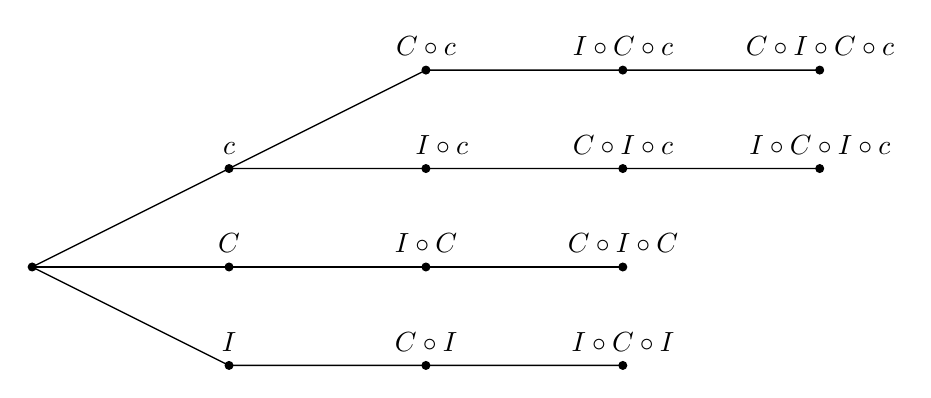
\begin{tikzpicture}
            \pgftransformscale{2.5}

            \def\offsetx{1};
            \def\offsety{0.5};
            
            \coordinate (A)     at (0, 0);          
            \coordinate (CA)    at (1, 0);
            \coordinate (ICA)   at (2, 0);
            \coordinate (CICA)  at (3, 0);
            \coordinate (IA)    at (1,-0.5);
            \coordinate (CIA)   at (2,-0.5);
            \coordinate (ICIA)  at (3,-0.5);
            
            \coordinate (cA)     at (0+\offsetx, 0+\offsety);          
            \coordinate (CcA)    at (1+\offsetx, 0.5+\offsety);
            \coordinate (ICcA)   at (2+\offsetx, 0.5+\offsety);
            \coordinate (CICcA)  at (3+\offsetx, 0.5+\offsety);
            \coordinate (IcA)    at (1+\offsetx, \offsety);
            \coordinate (CIcA)   at (2+\offsetx, \offsety);
            \coordinate (ICIcA)  at (3+\offsetx, \offsety);

            \draw[line width = 0.5pt] (A) -- (CA) -- (ICA) -- (CICA);
            \draw[line width = 0.5pt] (A) -- (IA) -- (CIA) -- (ICIA);
            \draw[line width = 0.5pt] (A) -- (cA) -- (IcA) -- (CIcA) -- (ICIcA);
            \draw[line width = 0.5pt] (cA) -- (CcA) -- (ICcA) -- (CICcA);
            
            \node[draw,circle,inner sep=1pt,fill] at (A) {};
            \node[label={$C$}, draw,circle,inner sep=1pt,fill] at (CA) {};
            \node[label={$I\circ C$}, draw,circle,inner sep=1pt,fill] at (ICA) {};
            \node[label={$C\circ I\circ C$}, draw,circle,inner sep=1pt,fill] at (CICA) {};
            \node[label={$I$}, draw,circle,inner sep=1pt,fill] at (IA) {};
            \node[label={$C\circ I$}, draw,circle,inner sep=1pt,fill] at (CIA) {};
            \node[label={$I\circ C\circ I$}, draw,circle,inner sep=1pt,fill] at (ICIA) {};

            \node[label={$c$}, draw,circle,inner sep=1pt,fill] at (cA) {};
            \node[label={$C\circ c$}, draw,circle,inner sep=1pt,fill] at (CcA) {};
            \node[label={$I\circ C\circ c$}, draw,circle,inner sep=1pt,fill] at (ICcA) {};
            \node[label={$C\circ I\circ C\circ c$}, draw,circle,inner sep=1pt,fill] at (CICcA) {};
            \node[label={[xshift=0.2cm]$I\circ c$}, draw,circle,inner sep=1pt,fill] at (IcA) {};
            \node[label={$C\circ I\circ c$}, draw,circle,inner sep=1pt,fill] at (CIcA) {};
            \node[label={$I\circ C\circ I\circ c$}, draw,circle,inner sep=1pt,fill] at (ICIcA) {};

          \end{tikzpicture}
          \caption{Lattice generated by $C, I, c$} 
    \end{figure}   

    There are exactly 14 points in this lattice so we have an upper bound of 14 on the number of distinct subsets which can be generated. To see that this upper bound is actually reached, consider the set
    \[
      A = (0,1)\cup(1,2)\cup\{3\}\cup([4,5]\cap \Q)
    .\] 
    It can be verified that this set satisfies the requirement, simply by plugging it into the lattice:
    \[
        \begin{aligned}
            A &= (0,1)\cup (1,2) \cup \{3\} \cup ([4,5]\cap \Q)\\
            I(A) &= (0,1)\cup (1,2)\\
            (C\circ I)(A) &= [0,2]\\
            (I\circ C\circ I)(A)&= (0,2)\\
            C(A) &= [0,2]\cup \{3\} \cup [4,5]\\
            (I\circ C)(A) &= (0,2)\cup (4,5)\\
            (C\circ I \circ C)(A) &= [0,2] \cup [4,5]\\
            c(A)&=(-\infty, 0]\cup\{1\}\cup [2,3)\cup (3,4)\cup ([4,5]\cap (\R-\Q))\cup (5,\infty)\\
            (I\circ c)(A)&= (-\infty,0)\cup(2,3)\cup(3,4)\cup (5,\infty)\\
            (C\circ I \circ c)(A)&=(-\infty,0]\cup[2,4]\cup [5,\infty)\\
            (I\circ C\circ I \circ c)(A)&=(-\infty, 0)\cup (2,4)\cup (5,\infty)\\
            (C\circ c)(A)&=(-\infty,0]\cup\{1\}\cup[2,\infty)\\
            (I\circ C\circ c)(A)&=(-\infty, 0)\cup (2,\infty)\\
            (C\circ I \circ C\circ c)(A)&=(-\infty, 0]\cup [2,\infty)
        \end{aligned}
    .\] 
\end{changemargin}

\end{document}
